\chapter{Antecedentes conceptuales}

\section{Trabajos relacionados}
%%copiado y pegado de la propuesta
Varios trabajos involucran el procesamiento de lenguaje natural en el ámbito de las ontologías~\cite{moreno2018ontologia}\cite{perez2002explotacion}\cite{vallez2009web}. Por un lado, existen herramientas que se enfocan en la verbalización de un conjunto de axiomas pertenecientes a una ontología, con el fin de generar un conjunto de sentencias que puedan ser utilizadas para reconocer la información perteneciente al dominio modelado, o documentar la ontología, utilizando lenguaje natural. En este tipo de trabajos se encuentran algunas herramientas como OntoVerbal~\cite{liang2013ontoverbal}, que utiliza la frecuencia con la que se utilizan conjuntos de axiomas para la descripción de entidades, y describe patrones lingüísticos para verbalizar los conjuntos de mayor frecuencia. Otra característica de OntoVerbal es que presenta en un mismo párrafo las sentencias que están estrechamente relacionadas. %Además, agrupa los axiomas alrededor de un tópico para crear párrafos. 
%Además, genera la creación de párrafos mediante la agrupación de axiomas alrededor de un tópico dado.

Por su parte, NaturalOWL~\cite{galanis2007generating}, se enfoca en la flexibilidad y fluidez del texto, agregando información lingüística a la ontología para verbalizar los axiomas.

Por otro lado, se han desarrollado herramientas para asistir durante el desarrollo de la ontología, permitiendo acceder a la información modelada en lógicas descriptivas en un formato de texto, y poder editarlo en lenguaje natural. Entre las herramientas desarrolladas se encuentran CLOnE~\cite{power2010complexity} y Aqualog~\cite{lopez2005aqualog},completamente orientadas a la comprensión de texto y no a la generación; y Attempto Tools~\cite{attempto}, que utiliza Attempto Controlled English  (ACE) que es un lenguaje natural controlado ~\cite{CNL}, para servir como lenguaje de representación de conocimiento, y de esta manera poder utilizar representaciones formales, sin necesidad de comprender la lógica interna. La ventaja de usar ACE radica en la posibilidad de generar lenguaje natural desde una representación de conocimiento en lógica, y viceversa.

Si bien estas herramientas cumplen con la verbalización de axiomas y asisten en el uso de ontologías evitando que los usuarios deban comprender las lógicas descriptivas y la sintaxis OWL, la comprensión de cada axioma aislado no asegura la comprensión del dominio completo. Un factor importante en la comprensión del dominio es la capacidad de relacionar los temas de manera coherente. La verbalización de axiomas es necesaria pero no suficiente para comprender las temáticas modeladas en la ontología. Existen conjuntos de axiomas que están relacionados y son complementarios para la descripción de entidades, y que expresados en conjunto como una unidad de información textual transmiten mejor la intención de ese conjunto de axiomas. OntoVerbal es la herramienta que tiene en cuenta este criterio, sin embargo, no planea una estructura de documento, por lo que no garantiza que el orden en el que aparezcan los párrafos maximice la coherencia.

En NaturalOWL se tiene en cuenta la calidad del texto de salida, pero compromete la representación del dominio, agregando información lingüística y ensuciando el dominio modelado. Por último en Attempto Tools se busca un equilibrio en la calidad del texto sin comprometer el dominio modelado, pero no se hace énfasis en la comprensión del dominio, ya que únicamente se traducen los axiomas en sentencias aisladas. 

Por estos motivo, en este trabajo se propone diseñar un algoritmo que agrupe la información relacionada a través de los temas principales presentes en la ontología. En este sentido, se propone una técnica alternativa a la de Reiter y Dale~\cite{reiter1997building} quienes realizan todo el ordenamiento de las sentencias e información involucradas en las últimas tareas de las verbalización. Por el contrario, en nuestra propuesta se pretende organizar la mayor parte de la información antes del proceso de verbalización en sí mismo, por considerarse que en éste punto es donde se puede lograr una manipulación más fácil y limpia de la información y dejando solamente el ordenamiento mínimo en etapas posteriores. De esta manera, esperamos que el resultado de la verbalización sean sentencias en lenguaje natural relacionadas semánticamente, que comprendan unidades textuales de mayor granularidad y no únicamente unidades textuales  aisladas (y posiblemente desordenadas) a nivel de oración  que cumplan una determinada sintaxis.

Con esto en mente, se propone diseñar e implementar una herramienta genérica para elegir, ordenar y generar un texto en lenguaje natural a partir de una ontología en OWL, con el fin de facilitar el entendimiento del dominio modelado, y asistir durante el proceso de modelado. Este trabajo hará foco principalmente en generación de texto en lenguaje español, y presentará un prototipo en lenguaje inglés.

\section{Generación de lenguaje natural}
\label{sec:tareas_gnl}
La generación de lenguaje natural es un proceso que tiene como principal objetivo la generación de texto a partir de datos de entrada.
Durante el proceso de generación de lenguaje natural, la entrada atraviesa diferentes etapas, a través de las cuales se modifica, hasta alcanzar la última etapa en la que se obtiene un el resultado en lenguaje natural.

Según el tipo de entrada, un Sistema de Generación de Lenguaje Natural (SGLN) puede clasificarse en Datos a Texto o Texto a Texto~\cite{vicente2015generacion}.
\begin{itemize}
    \item Datos a Texto: la entrada es un conjunto de datos estructurados. Por ejemplo, pueden ser datos numéricos, tal como la descripción del clima; datos  tabulares~\cite{mahapatra2016statistical}; datos en formato JSON\footnote{referencia a tesis matias?}; o estructuras más complejas como ontologías.
    \item Texto a Texto: la entrada puede ser texto u oraciones aisladas. Para trabajar con este tipo de entrada, se utilizan enfoques estadísticos~\cite{mittal1999ultra}; la transformación del texto a estructuras de datos~\cite{saldanha2004creation}; o modelos formales~\cite{guo2018long}.
\end{itemize}

\subsection{Tareas de la generación de lenguaje natural}
En el ámbito de la Generación de Lenguaje Natural, se engloban las tareas de cada nivel de abstracción en una etapa particular. Existen tres etapas principales: \emph{macro planning}, \emph{micro planning} y \emph{realización gramatical}~\cite{vicente2015generacion}.

\begin{itemize}
    \item  \emph{Macro planning:} agrupa las tareas de nivel más abstracto. Se encarga de seleccionar la información que se usará en la generación de texto y de organizarla a nivel de capítulos, secciones, párrafos, y sentencias.
    \item \emph{Micro planning:} es la etapa asociada a la construcción de sentencias, agrupa las tareas de nivel de abstracción intermedio. Dado un conjunto de datos que deben estar presentes en una sentencia, el \emph{micro planning} decide en qué orden aparecerán y cómo se combinarán para producir una oración cohesiva. 
    Para esto, se selecciona las configuraciones léxicas de las palabras, se elige qué entidades se reemplazarán por una expresión de referencia, y qué oraciones se pueden combinar para mejorar la fluidez del texto.
    \item \emph{Realización gramatical y expresiones de referencia:} es la última etapa, donde se seleccionan las palabras adecuadas según lo establecido en el \emph{micro planning}. Puede involucrar, por ejemplo, el uso de algoritmos de conjugación de verbos. Expresiones de referencia se refiere a la descripción de objetos.
\end{itemize}

\subsection{Arquitecturas de SGLN}
%https://pdfs.semanticscholar.org/bfc1/44401be9cb93493b0974afb561b8d3c2d1ec.pdf
La forma en que se comunican las tareas descritas en la Sección anterior definen la arquitectura del sistema~\cite{ibanez2004arquitectura}. La arquitectura más generalizada es el \emph{pipeline}~\cite{hervas2008descripcion}, representado en la Figura \ref{fig:arq_pipeline}.
%https://pdfs.semanticscholar.org/6cd2/54a9a4ea49aee61c3add58c11c29162428ae.pdf
Esta arquitectura tiene la ventaja de ser simple de implementar, pero es poco flexible, por lo que las decisiones tomadas en etapas tempranas deben mantenerse a lo largo del pipeline sin posibilidad de mejora.

\begin{figure}
    \centering
    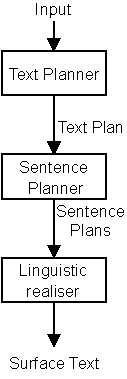
\includegraphics[]{img/antecedentes/pipeline.pdf}
    \caption{Arquitectura pipeline}
    \label{fig:arq_pipeline}
\end{figure}
 

Cada arquitectura se enfoca en dos aspectos fundamentales: la independencia de los módulos (qué tan acoplado/desacoplado está el sistema) y el flujo de control entre ellos. Desde el punto de vista de la separación de los módulos, se pueden encontrar arquitecturas integradas (o monolíticas) donde todo el sistema está formado por un único módulo, hasta sistemas en los que a cada tarea se le asocia un módulo separado~\cite{hervas2008descripcion}. Desde el punto de vista del flujo de control, se encuentran arquitecturas como pipeline donde la información fluye en un único sentido a través de los módulos, hasta arquitecturas de pizarra, donde la información se escribe en un sitio en común a todos los módulos.

Una descripción más detallada de cada arquitectura se encuentra  en~\cite{ibanez2004arquitectura}.

\subsection{Enfoque para abordar la GNL: coherencia local y global}
En la generación de texto automática, además de desear cumplir ciertas características léxicas y sintácticas del lenguaje destino, se requiere que el texto sea coherente. Para alcanzar esta coherencia textual, se puede dividir el estudio de coherencia en dos: la coherencia local, asociada a la conexión semántica entre oraciones; y la coherencia global, asociada al asunto del texto~\cite{van2005estructuras}.

Para abordar el problema de la coherencia local, nos basaremos en lo postulado por la Teoría de Centrado~\cite{grosz1986towards}.

En cuanto a la coherencia global, utilizaremos como recurso a la Teoría de Veins~\cite{cristea1998veins}.

\subsubsection{Teoría de Centrado}
La Teoría de Centrado es una teoría de coherencia local y saliencia de discurso. Por un lado, intenta caracterizar los discursos coherentes entre entidades, teniendo en cuenta la forma en la que se introducen y discuten sus entidades. Por otro lado, se encarga de predecir qué entidades serán más destacadas en un momento dado~\cite{poesio2004centering}.

Esta teoría propone un conjunto de reglas, que de aplicarlas favorece la coherencia del discurso. La afirmación más fundamental de la Teoría de Centrado es que, en la medida en que un discurso se adhiera a las restricciones centrales, su coherencia aumentará y la carga de inferencia sobre el oyente disminuirá~\cite{kruijff1997topics}. Esta característica que aclama, resulta conveniente para el objetivo que busca nuestro trabajo, respecto a minimizar los esfuerzos de un usuario para comprender el dominio modelado en una ontología.

Según~\cite{vicente2015generacion}, ``Un elemento de una parte del discurso a nivel local se constituye como el foco de atención o centro de ese contexto, como la entidad más relevante a la que se refiere el resto de proferencias.''. Desde el punto de vista de la lingüística computacional, esto resulta útil para abordar el problema de la anáfora\footnote{Una anáfora es una figura retórica que consiste en la repetición de una o varias palabras al principio de un verso o enunciado.}. 

\subsubsection{Teoría de Veins}
La Teoría de Veins es una extensión de la Teoría de Centrado. Esta teoría propone un modelo para la descripción de la coherencia global. La estructura jerárquica del texto permite la relación (a través de referencias) entre unidades textuales aún cuando no se encuentran en una disposición lineal~\cite{cristea2005motivations}, garantizando que se mantiene la coherencia del texto.

\section{Teoría de grafos}
La teoría de grafos se encarga de estudiar las propiedades de los grafos. Un grafo es una estructura de datos que consiste de un conjunto de vértices conectados por un conjunto de arcos que pueden ser usados para modelar relaciones entre los objetos en una colección~\cite{mihalcea2011graph}.

Algunos aspectos que se estudian de los grafos son su estructura (jerárquica, árbol, conexos, bipartitos, etc.), las medidas de sus nodos (centralidad relativa, absoluta~\cite{freeman1978centrality}), los algoritmos de recorridos (profundidad, anchura, etc.), etc.

La teoría de grafos tiene diversas aplicaciones, por ejemplo el análisis de redes sociales, representación de mapas conceptuales, diseño de circuitos eléctricos, topologías de redes de computadoras, etc. Actualmente se estudia la teoría de grafos y el procesamiento de lenguaje natural en conjunto, para hallar solución a diferentes problemas del procesamiento de texto, como el etiquetado léxico, clasificación de texto y clustering~\cite{mihalcea2011graph}, desambiguación semántica de palabras~\cite{MihalceaSinhaDisambiguation}\cite{ArabJahromiDisambiguation}, extracción de keywords~\cite{Litvak:2008:GKE:1613172.1613178}\cite{beliga2015overview}, generación de resúmenes~\cite{plaza2011uso}, entre otras.

\subsection{Criterio de centralidad de un nodo}
El criterio de centralidad es alguna función del grado de un nodo~\cite{freeman1978centrality}. El grado de un nodo $n$ es la cuenta de la cantidad de nodos adyacentes a $n$. 

La medida de centralidad es utilizada para cuantificar la importancia de un nodo~\cite{2018transfer}. Un ejemplo del cálculo de centralidad es \emph{PageRank}~\cite{page1999pagerank} el algoritmo utilizado por Google para calcular la relevancia de los documentos web.

Existen diferentes medidas de centralidad, algunas de ellas son:
\begin{itemize}
    \item \emph{Degree Centrality}: en grafos no dirigidos es la cuenta de la cantidad de conexiones de un nodo; en un grafo dirigido, se tiene en cuenta la dirección de la conexión, siendo outdegree la medida de la cantidad de conexiones de salida de un nodo, e indegree la medida de la cantidad de conexiones entrantes al nodo. 
    \item \emph{Closeness Centrality}: es la longitud promedio del camino más corto entre el nodo y todos los demás nodos en el grafo.
    \item \emph{Between Centrality}: calcula la cantidad de veces que un nodo actúa como un puente en el camino más corto entre otros dos nodos.
\end{itemize}

\subsection{Algoritmos de recorridos de grafos}
Se utilizan para recorrer los nodos de un grafo. Dos clasificaciones principales:
\begin{itemize}
    \item Recorrido en profundidad: dado un nodo $n$, se visita un nodo $n'$ adyacente, explorando cada camino que salga de él. Hasta que no se haya finalizado de explorar uno de los caminos no se comienza con el siguiente. Un camino deja de explorarse cuando se llega a un nodo ya visitado. 
    \item Recorrido en anchura: dado un nodo $n$, se visitan todos sus nodos adyacentes. Sea $n'$ un adyacente de $n$, no se visita ningún adyacente de $n'$ hasta que ya se hayan visitado todos los adyacentes de $n$. 
\end{itemize}

\section{Procesamiento de lenguaje natural y teoría de grafos}
La representación de texto como una estructura de datos basada en grafos ha sido usada para dar soporte a las tareas de procesamiento de lenguaje natural. En TextGraph Workshop Series\footnote{http://www.textgraphs.org} se pone a disposición una plataforma para el intercambio de ideas que beneficien ambos campos de investigación. 

La representación de datos como un grafo beneficia el PNL poniendo a disposición los algoritmos conocidos, permitiendo la navegación del grafo para extraer y clasificar el contenido. Algunas tareas de PLN que son resueltas utilizando grafos son la creación de resúmenes~\cite{mihalcea2004graph}\cite{erkan2004lexrank} y minería de texto~\cite{Jin:2007:GTR:1244002.1244182}\cite{beliga2015overview}.

\begin{itemize}
    \item Resúmenes: ``La generación automática de resúmenes consiste en la creación de una versión reducida de uno o varios documentos por parte de un programa de ordenador, de tal forma que el resumen producido condense la información importante del texto de entrada''~\cite{plaza2011uso}.
    \item Minería de texto: ``Es el proceso de extracción automática de información fundamental de textos,  detección  automática  de temas  predominantes en un conjunto de documentos y búsqueda de textos relevantes mediante consultas de grandes prestaciones y flexibilidad''~\cite{brun2004articulo}.
\end{itemize}

\section{Ontologías y teoría de grafos}
Tanto en la academia como en la industria~\cite{soylu2018navigating} se han utilizado grafos para la representación de conocimiento. Este enfoque permite explotar las propiedades de un grafo dentro del área de la visualización de la información, por ejemplo para la representación y navegación de ontologías~\cite{escarza2005visualizacion}.

El uso de herencia múltiple en ontologías genera estructuras de datos en forma de grafos dirigidos, sin embargo se pueden usar diferentes criterios para mostrar el contenido de una ontología, por ejemplo Protégé utiliza una visualización en forma de árbol para mostrar la jerarquía de clases, donde cada nodo del árbol es una clase~\cite{protegehierarchy}. Como es posible que un nodo sea hijo de más de un padre, existe redundancia en la visualización, ya que un nodo puede repetirse en dos ramas diferentes.

En~\cite{mellish2008natural} presentan una investigación acerca de \emph{Natural Language Directed Inference from Ontologies} (NLDI), en el cual buscan determinar el contenido para describir una entidad presente en una ontología. Los axiomas elegidos para tal descripción surgen de aplicar un algoritmo \emph{best-fist search} sobre un grafo generado a partir de los axiomas de la ontología.

En~\cite{crampes2007ontology} comparan dos aplicaciones que utilizan ontologías para soportar y dirigir la navegación conceptual. En ellas, aplican criterios de selección y ordenamientos de conceptos a partir de las relaciones de las entidades en la ontología del dominio y de reglas específicas de una ontología pedagógica. 

De estos trabajos se observan dos aspectos importantes para integrar la teoría de grafos y la representación de las ontologías:
\begin{itemize}
    \item Determinar qué información de la ontología será usada para crear los nodos y los enlaces del grafo.
    \item Establecer un método de navegación del grafo.
\end{itemize}

Dado que se trabaja con grafos semánticos, en el contexto de la generación de lenguaje natural es deseable aprovechar al máximo la semántica de las relaciones, ya que cada ruta entre los axiomas corresponden a diferentes transiciones posibles en un texto coherente~\cite{mellish2008natural}.
